\section{シミュレーション結果}
本実験( TODO: ?)では, 作成したシミュレータを用いてHodgkin-Huxleyモデルの神経細胞モデル( TODO: ref)からなる( TODO: 章番号)で示したベンチマークネットワークを最適化しシミュレーションを行い,
その後シミュレーションの結果を用いて最適化に用いたパラメータを定量的に評価する.\\
本論文執筆時においてパラメータの探索は全探索を用いているため, パラメータすべての組み合わせを大規模なシミュレーションで行うことは現実的ではない.
そのため, (  TODO: アルゴリズムの説)で述べたように, 実行マシンに関わるパラメータ(プロセス数とスレッド数)は並列実行に関連するものであり,
モデルに関わるパラメータ(SIMD化と配列のくくり出し)は逐次実行に関するものであるという事実を利用する.\\
5.1節では, シミュレーション時間をスパイクが出始める100msに設定したシミュレーションを3回行い,
その平均をとった実行時間を用いてパラメータの評価を行い, 大規模のシミュレーションを行う際に除外できるパラメータ候補の解析を行う.\\
5.2節から5.5節においては, それぞれのパラメータに対して規模の変更を通してより詳細なシミュレーションを行う.\\
5.6節においては, それまでの結果を利用しNEURONのデフォルトと手動での最適化を図ったシミュレーションとの比較を行う.\\
また, コンパイラについては京環境でICCを利用することができなかったため, クラスタ環境上でのみシミュレーションを行い,
最適化の指標の一つとするにとどまった.\\

\subsection{小規模シミュレーションでのパラメータ比較}
本節では, ベンチーマクモデルの中で実際の神経回路ネットワークと最も近いと考えられるWatts and Strogatzネットワークに対して
以下のパラメータを用いてシミュレーションを行った.\\
\subsubsection{クラスタ環境}
\begin{table}[htb]
  \caption {クラスタでのパラメータ}
  \begin{center}
    \begin{tabular}{|c|p{12cm}|}
      \hline
      パラメータ & 値の範囲\\ \hline
      ノード数 & 1\\ \hline
      MPIプロセス数 & 1〜28\\ \hline
      OpenMPスレッド数 & 1〜16\\ \hline
      SIMD化 & 行う or 行わない\\ \hline
      配列のくくり出し & 行う(SIMD化を行っているならば) or 行わない\\ \hline
    \end{tabular}
  \end{center}
\end{table}
プロセス数についてはクラスタでのコア数の上限まで,
スレッド数についてはNEURONの内部で細胞単位でスレッド並列を行う上限を16と設定していたためその16を上限として設定した.\\
また, 配列のくくり出しに関してはSIMD化の過程で変数を配列化する必要があるため, SIMD化をした上で行うか否かという条件とした.\\

\paragraph{MPIプロセス数}

\paragraph{OpenMPスレッド数}

\paragraph{逐次最適化}



\clearpage
\subsubsection{京環境}
\begin{table}[htb]
  \caption {京でのパラメータ}
  \begin{center}
    \begin{tabular}{|c|p{12cm}|}
      \hline
      パラメータ & 値の範囲\\ \hline
      ノード数 & 8\\ \hline
      MPIプロセス数 & 1〜8\\ \hline
      OpenMPスレッド数 & 1〜16\\ \hline
      SIMD化 & 行う or 行わない\\ \hline
      配列のくくり出し & 行う(SIMD化を行っているならば) or 行わない\\ \hline
    \end{tabular}
  \end{center}
\end{table}

\subsection{MPIプロセス数}
\begin{figure}[h!]
% h:here, t:top, b:bottom, p:page
%  \begin{left}
%    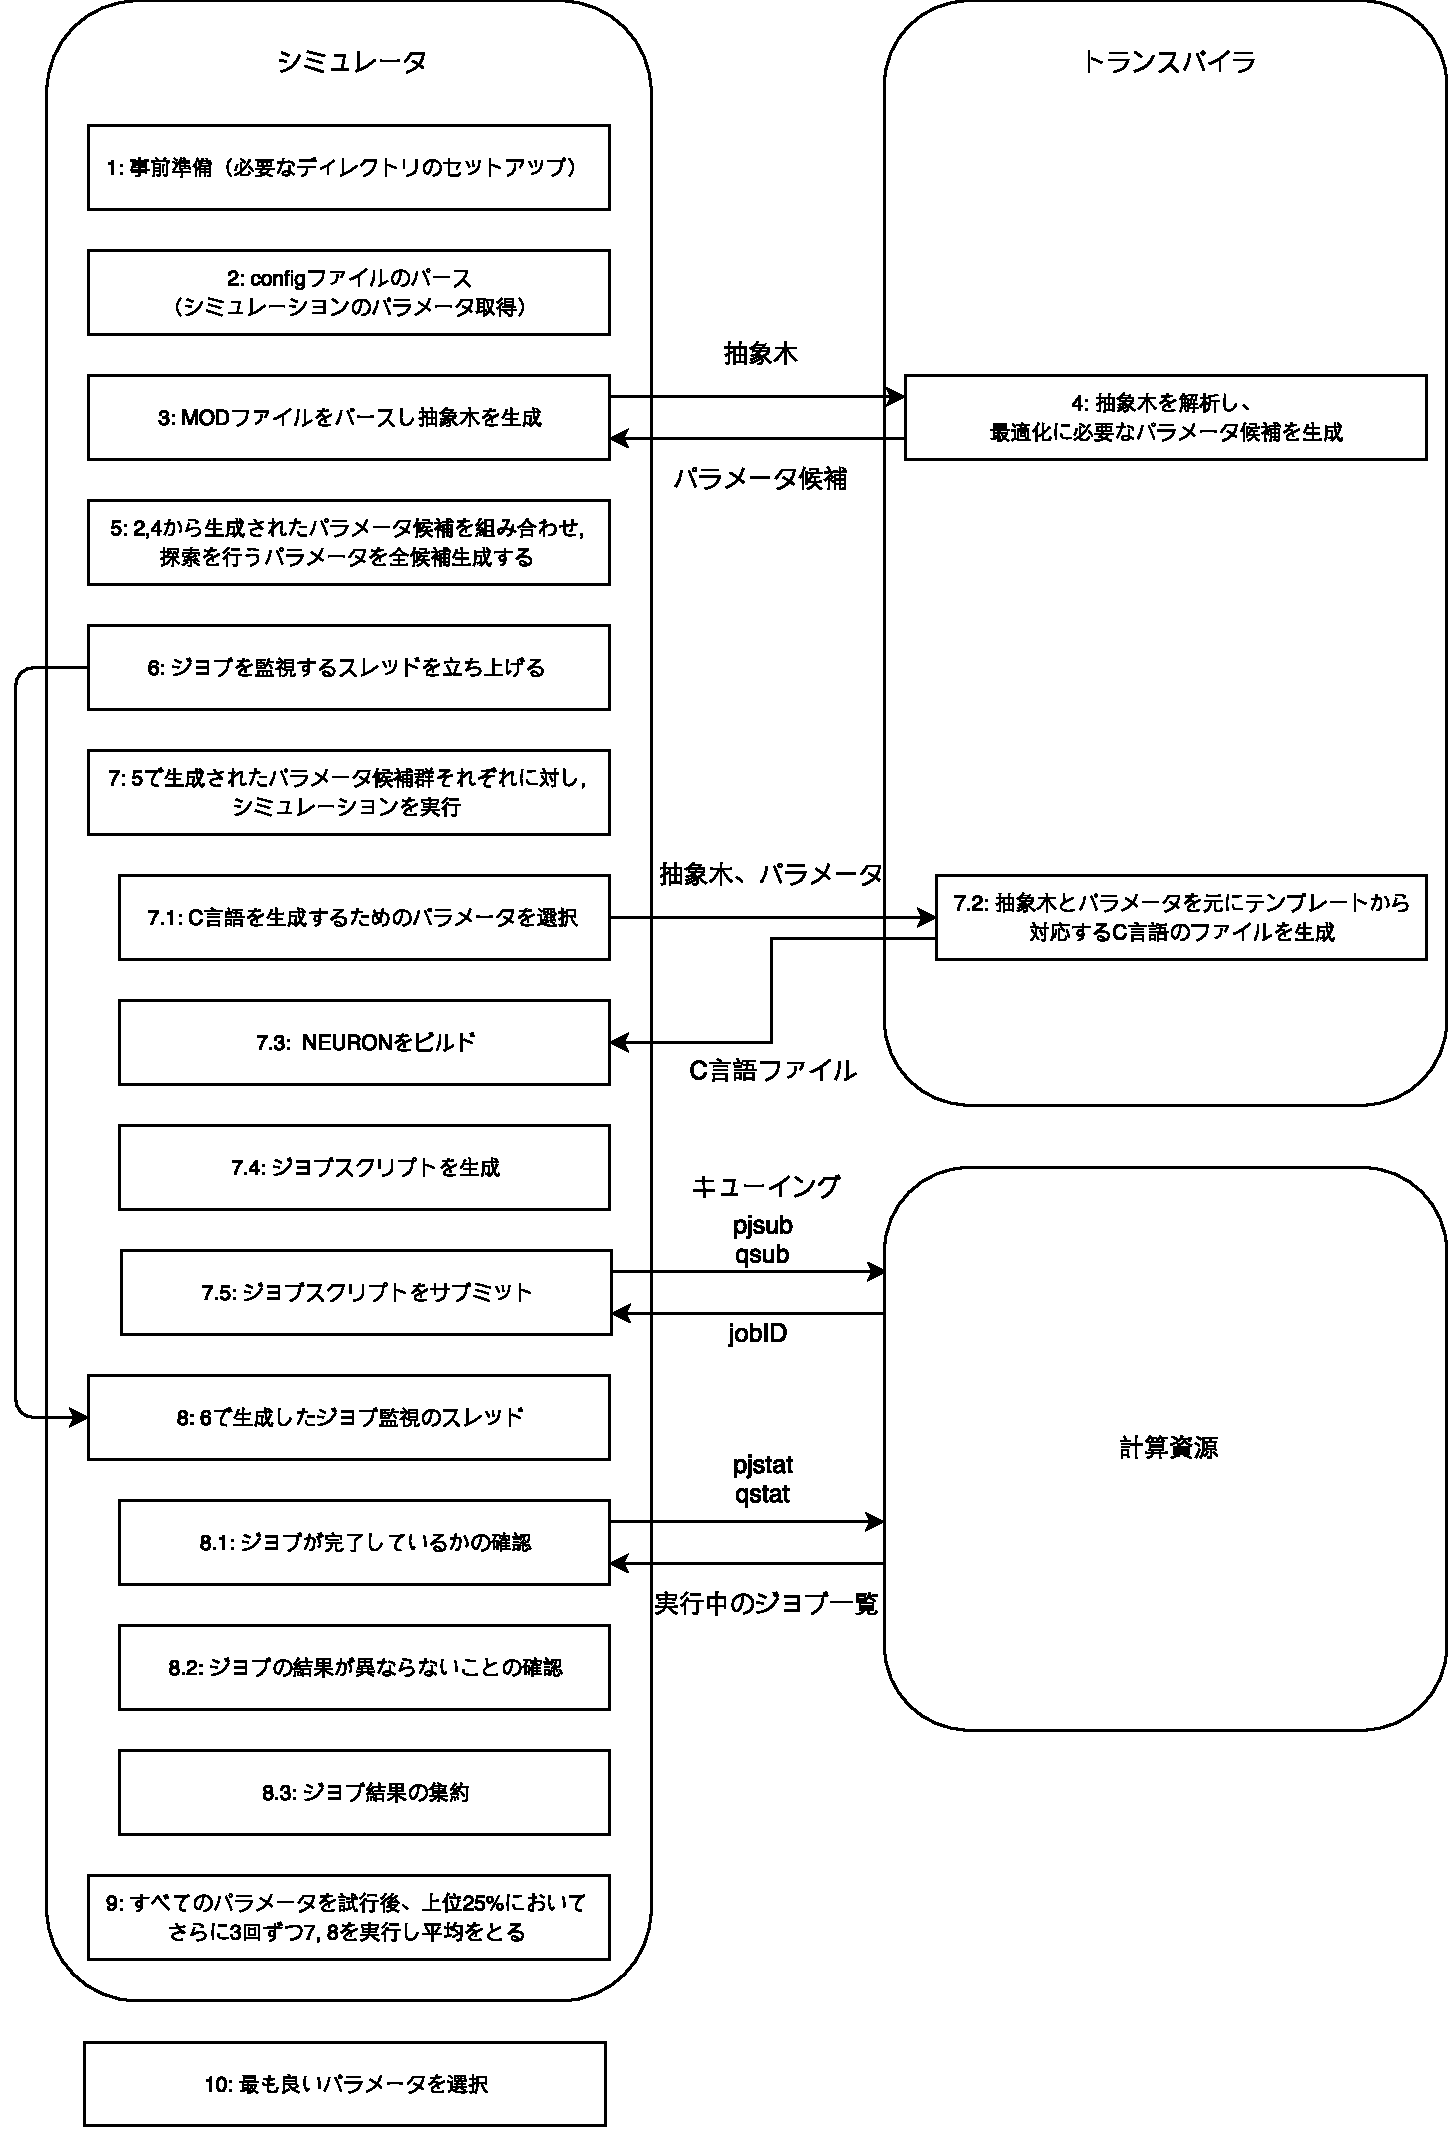
\includegraphics[width=18.0cm]{./images/Genie.pdf}
    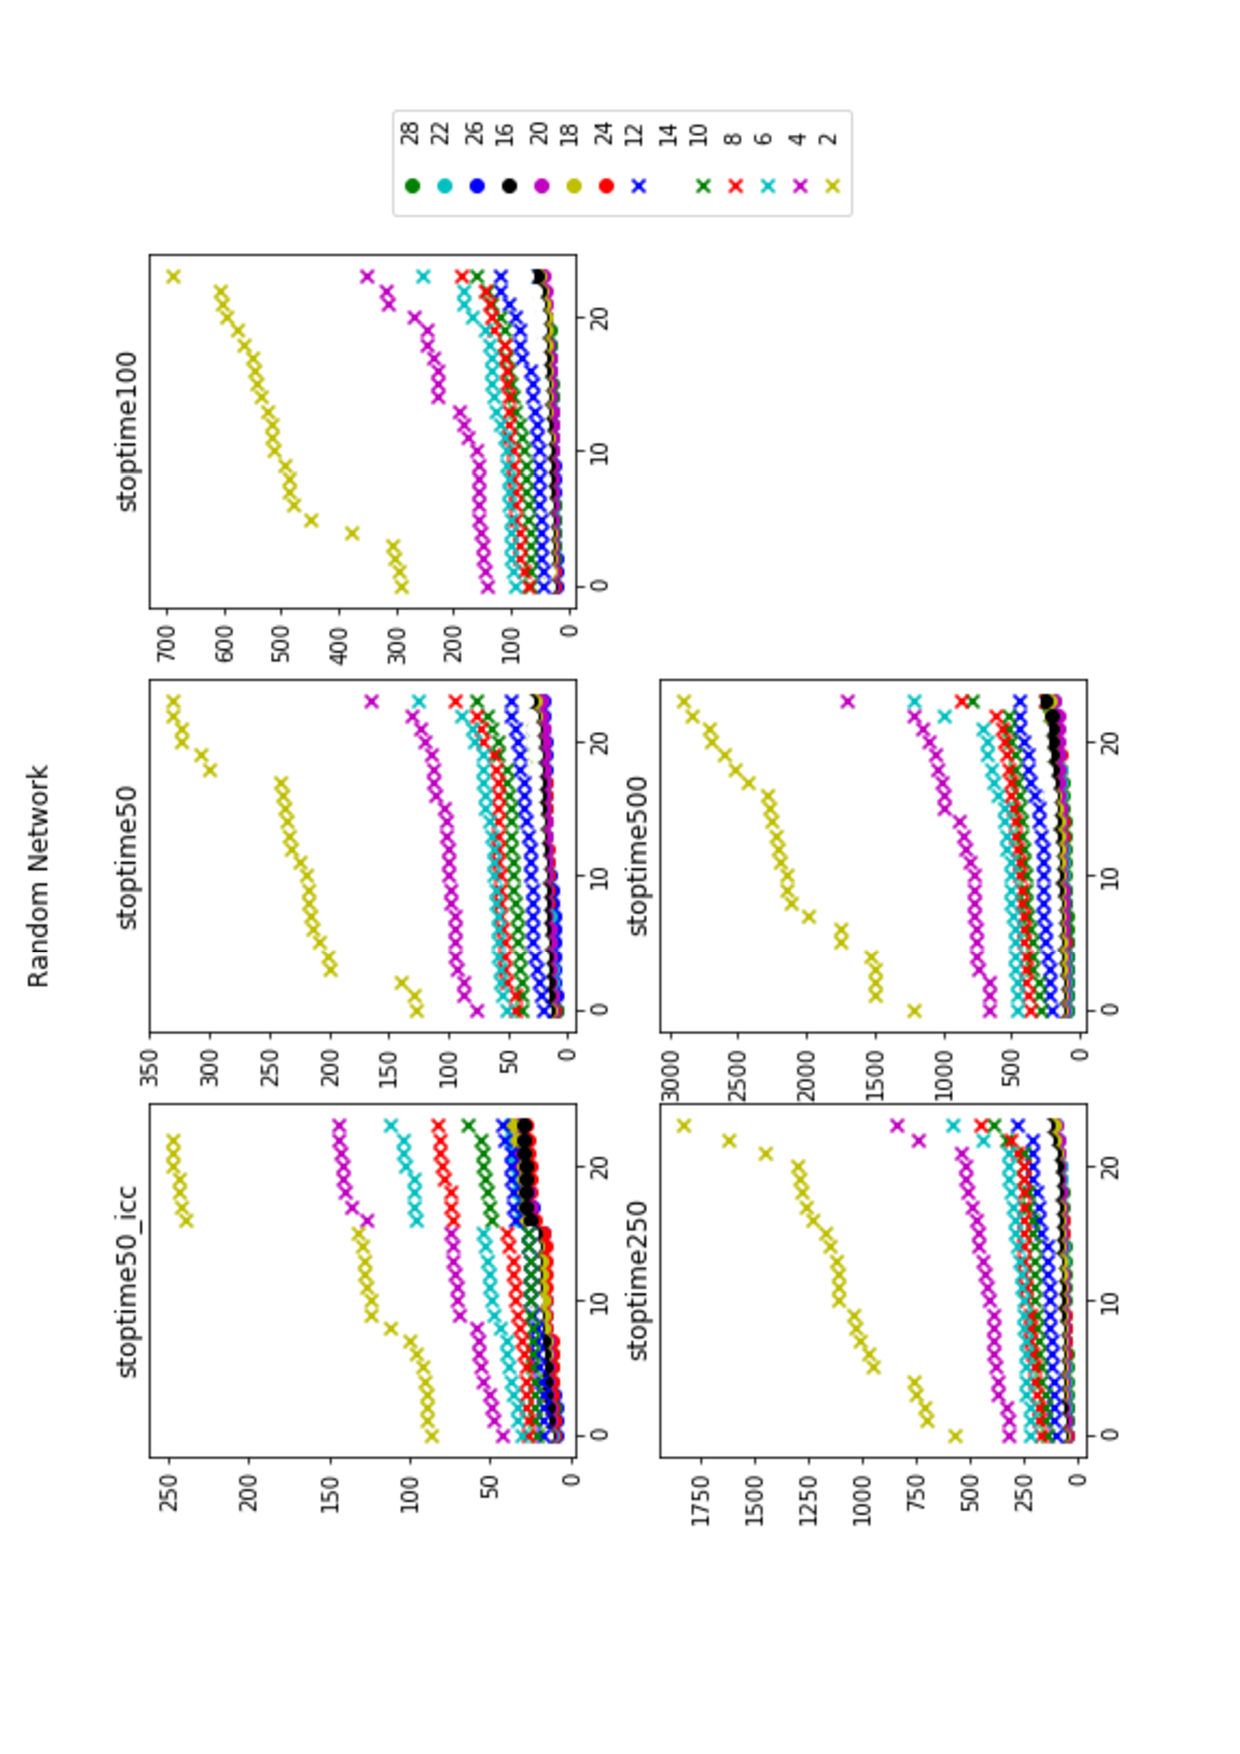
\includegraphics[width=0.9\textwidth, angle=-90]{./images/random-network.pdf}
    \caption{ランダムネットワーク}
    \label{fig:bench-network}
%  \end{left}
\end{figure}
\subsection{OpenMPスレッド数}

\subsection{SIMD化}

\subsection{配列のくくり出し}

\subsection{最適化結果の比較}
